\documentclass[a4paper,fontsize=9pt, DIV=calc]{scrartcl}
\usepackage[utf8]{inputenc}
\usepackage[light,condensed,math]{kurier}
\usepackage[default]{sourcesanspro}
\usepackage{zi4}
\usepackage[T1]{fontenc}
\usepackage[ngerman]{babel}
\usepackage{amsmath}
\usepackage{amsfonts}   
\usepackage{amssymb}
\usepackage{multicol}
\usepackage[activate={true,nocompatibility},final,tracking=true,kerning=true,spacing=true,factor=1100,stretch=10,shrink=10]{microtype}
\usepackage{geometry}
\usepackage[pdftex]{graphicx}
\usepackage[usenames]{color}
\usepackage{boxedminipage}
\usepackage{fancybox}
\usepackage{multirow}
\let\chapter\section
\usepackage[ruled,vlined,linesnumbered]{algorithm2e}
\usepackage{rotating}
\usepackage{polynom}
\geometry{a4paper,left=20mm,right=20mm, top=5mm, bottom=5mm} 
\usepackage{multicol}
\usepackage{setspace}
\usepackage{parskip}
\usepackage{listings} % Listings
\usepackage[stable]{footmisc}
\usepackage{tikz}
\usetikzlibrary{arrows,shapes}
\usetikzlibrary{positioning}
\usepackage{pdflscape}
\usepackage{amsthm}
\usepackage{thmtools}
\usepackage{fix-cm}
\usepackage{wrapfig}
\usepackage{float}
\usepackage{enumitem}
\usepackage{epstopdf}

\usepackage{titlesec}
\usepackage[colorlinks=false, pdfborder={0 0 0}]{hyperref}

\definecolor{seccol}{rgb}{0,0.8,0.3}

\titlespacing{\section}{0pt}{*0}{*0}
\titlespacing{\subsection}{0pt}{*0}{*0}
\titlespacing{\subsubsection}{0pt}{*0}{*0}

\declaretheoremstyle[
    spaceabove=1em, spacebelow=2em,
    headfont=\normalfont\bfseries,
    notefont=\normalfont\bfseries, notebraces={(}{)},
    bodyfont=\normalfont
]{defstyle}

\declaretheoremstyle[
    spaceabove=1em, spacebelow=2em,
    headfont=\normalfont\bfseries,
    notefont=\normalfont\bfseries, notebraces={(}{)},
    bodyfont=\normalfont,
    headpunct=\newline
]{defstyle}



\declaretheorem[style=defstyle]{definition}
\declaretheorem[style=defstyle, name=Satz]{satz}
\declaretheorem[numbered=no]{beweis}
\declaretheorem[name=Beispiel]{beispiel}




\newcommand{\is}{=}
\newcommand{\true}{$1$}
\newcommand{\false}{$0$}

% Colors
\definecolor{grey}{rgb}{0.2, 0.2, 0.2} 
\definecolor{lightgrey}{rgb}{0.9, 0.9, 0.9} 

\definecolor{siemensyellow}{cmyk}{0.01, 0.08, 0.92, 0.01}
\definecolor{siemensblue}{cmyk}{0.94, 0.63, 0.03, 0.05}
\definecolor{siemensred}{cmyk}{0.02, 0.94, 0.90, 0.06}
\definecolor{siemensorange}{cmyk}{0.01, 0.57, 0.91, 0.02}
\definecolor{siemenscoolgrey}{cmyk}{0.55, 0.31, 0.25, 0.02}
\definecolor{siemensgreen}{cmyk}{0.83, 0.03, 0.93, 0.06}




% Listings

%\setlength  {\parindent} {0em}  %Kein Einrücken
\renewcommand\lstlistingname{Quellcode} % Umbenennung der Listings in Algorithm
\renewcommand\lstlistlistingname{Quellcode} % Umbenennung von Listings in Code


\columnseprule=0.2pt
\columnsep=2mm


\title{Softwarearchitektur}
\subtitle{Zusammenfassung}
\author{Thomas Vierthaler\footnote{besten Dank an Mateo Luzi für die Idee mit der skalierbaren Schrift!} (Basis von Michael Dorner)}
\date{\today}

\begin{document}

\lstdefinestyle{siemens} {
	%language		= C++,
	basicstyle		= \ttfamily\small,
	identifierstyle	= \ttfamily\normalsize,
	stringstyle		= \ttfamily\small\color{siemensred},
	commentstyle	= \ttfamily\small\color{siemensgreen},
	keywordstyle	= \ttfamily\small\color{siemensblue},
	columns			= fullflexible,
	showstringspaces= false,
	emphstyle 		= \color{siemensorange},
	frame			= single,
	morekeywords	= {REFERENCES, DATETIME},
	emph			= {Michi},
	framesep 		= 2pt,
	rulesep			= 0pt,
	framerule		= 0.25pt,
	captionpos		= b,
	%linewidth		= 0.75\textwidth,
	xleftmargin 	= 2pt,
	xrightmargin	= 2pt,
	aboveskip		= 1pt,
	belowskip		= 2pt
 }



\setlength{\parindent}{0pt} 

\renewcommand{\arraystretch}{0.9}


\maketitle
\tableofcontents
\clearpage
\newgeometry{left=1mm,right=1mm, top=1mm, bottom=1mm}
\begin{multicols}{2}
\section{Allgemeines}
\subsection[Prinzipien der Softwaretechnik]{Prinzipien der Softwaretechnik}

\vspace{-0.5em}
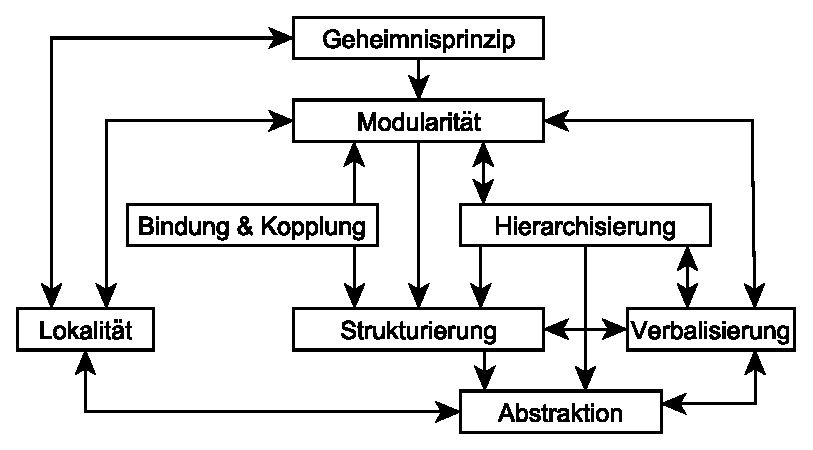
\includegraphics[scale=0.72]{src/abhaengigkeiten}
\begin{flushright}
    \vspace{-6.5cm}
    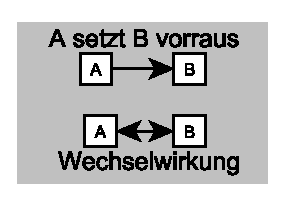
\includegraphics[scale=0.70]{src/legende_abh}
    \vspace{4cm}
\end{flushright}


\begin{description}[leftmargin=*]\itemsep-2mm
    \item[Abstraktion] ist die Verringerung der Komplexität durch Vernachlässigung von Nebenaspekten und Details. Ein Modell erfüllt die 3 Merkmale: 
		\begin{description}[leftmargin=*]\itemsep-2mm
		\item[Abbildungsmerkmal] bildet etwas real oder fiktiv existierendes ab, mit Realitätsbezug
		\item[Verkürzungsmerkmal] hebt Wesentliches hervor, lässt Unwesentliches weg
		\item[Pragmatisches Merkmal] kann unter best. Bedingungen Original ersetzen
		\end{description}
    \item[Strukturierung] ein komplexes System eine reduzierte Darstellung zu finden, die den Charakter des Ganzen mit seinen spezifischen Merkmalen widergibt.

		\item[Dekomposition] Stepwise Refinement Prinzip: Komplexes Problem wird zerteilt in einfachere Unterprobleme (Rekursiv, bis klar und lösbar).
		
		\item[Wiederverwendung] möglich, wenn technische, organisatorische und Management Voraussetzungen erfüllt sind. Erhöht Aufwand bei Erstellung (ca. 60\%) durch Dokumentation, Testaufwand, Archivierung und Wartung.
		 \item[Verbalisierung] bedeutet, Gedanken und Vorstellungen in Worten auszudrücken und damit ins Bewußtsein zu bringen. Gute Verbalisierung erreicht man durch aussagetechnische und einprägsame Namensgebung, geeigneten Kommentaren und selbstdokumentierende Konzepte.
		
		\item[Hierarchisierung] ist die Zuordnung einer Rangordnung der Elemente eines Systems. Elemente gleicher Rangordnung bilden eine Hierarchieebene. Hierarchisierung lässt sich dem Prinzip der Strukturierung unterordnen, weshalb auch die Vorteile der Strukturierung gelten, wobei eine Hierarchie stärker einschränkt als einer Struktur.
				
		\item[Standardisierung] erfolgt durch die Anwendung von Richtlinien, Normen, Guidelines,... und betrifft die unterschiedlichsten Bereiche:
				Namensvergabe und Pflichtenheftgestaltung, Verwendung von Standardgliederungen bei der Dokumentenerstellung, Einhaltung von Programmierstandards, Oberflächenstandards (Masken, Listen,...), Einheitliches Fehlermanagement, Einheitliche Verwendung von Funktionstasten

    \item[Modularisierung] Zusammensetzung eines Systems aus einzelnen Bausteinen, mit den Eigenschaften: Kohärenz, Kontextunabhängigkeit, Schnittstellenspezifikation, Information Hiding, Lokalitätsprinzip und lose Kopplung. Sie ist eng mit Abstraktion verknüpft, da die Modularisierung gleichzeitig das Bilden von Abstraktionsebenen erfordert.
		\begin{description}[leftmargin=*]\itemsep-2mm
		\item[Verbesserung/Erleichterung von] Änderungsfreundlichkeit, Wartbarkeit, Standardisierung, Arbeits- Organisation und Planung, Überprüfbarkeit
		\end{description}
				
		\item[Kohärenz] (Kohäsion, feste Bindung) Module sollen eine klar umrissene Verantwortung für eine (fachliche/technische) Aufgabe besitzen, d.h. alle Funktionen stehen in starkem Zusammenhang. Idealerweise realisert ein Modul eine Verantwortung. (Kohärenz heißt, möglichst viele Abhängigkeiten \textbf{in} einem Modul)
		\item[Lose Kopplung] Abhängigkeiten zwischen Modulen sollen minimal sein. Jedes Modul soll möglichst wenig andere kennen. Die Zahl und Komplexität der Schnittstellen zwischen ihnen sind auf ein Minimum zu reduzieren. (Lose Kopplung bedeutet, möglichst wenige Abhängigkeiten \textbf{zwischen} Modulen)

		\item[Kontextunabhängigkeit] bedeutet, dass ein Modul unabhängig von seiner Umgebung entwickelbar/übersetzbar/prüfbar/wartbar/verständlich ist.
		
		\item[Schnittstellenspezifikation] ist der Name für das Prinzip, dass beschreibt, dass jedes Modul eine klar umrissene Verantwortung für eine fachliche oder technische Aufgabe besitzen soll.
		
    \item[Geheimnisprinzip] bedeutet, dass es für den Benutzer eines Moduls nicht ersichtlich ist, welche implementierungsabhängigen Interna verwendet wurden. Es sollte immer im Zusammenhang mit der Modularisierung verwendet werden. Vorteile sind:
		\begin{description}[leftmargin=*]\itemsep-2mm
		\item[Datenkonsistenz] interner Daten kann besser sichergestellt werden, da direkte, unkontrollierbare Manipulationen nicht möglich sind
		\item[Benutzung einer Systemkomponente / eines Subsystems] wird zuverlässiger, da nur Schnittstelle benutzt werden kann und wird nicht mit unnötigen Informationen belastet.
		\item[Jedoch] muss die Schnittstelle vollständig und exakt beschrieben werden.
		\end{description}
		\item[Lokalisierung] alle zur Lösung eines Problems oder zur Einarbeitung in einen Bereich benötigten Informationen sind an einer Stelle zu finden.		
				\begin{description}[leftmargin=*]\itemsep-2mm
				\item[Vorteile] Ermöglicht schnelle Einarbeitung, fördert Verständlichkeit und Lesbarkeit und erleichtert Wartbarkeit und Pflege.
				\item[Nachteile] Erschwert Geheimnisprinzip, da öffentlich zugängliche Daten und private Informationen getrennt werden müssen, obwohl sie inhaltlich zusammengehören und daher an einer lokalen Stelle zusammenstehen sollten.
				\end{description}
\end{description}

\begin{description}[leftmargin=*]\itemsep-2mm
\item[Design Structure Matrix] horizontale Richtung: Parameter A \textbf{wird beeinflusst} von X, Y, Z. Vertikale Richtung: Parameter A \textbf{beeinflusst} T, U, V. Es können sich sequentielle und gegenseitige Abhängigkeiten ergeben.
\item[Task Structure Matrix] ist Equivalent zur DSM, zeigt dabei noch die Reihenfolge in welcher die Elemente implementiert werden sollen
\item[Design Rules] sind Rahmenbedingungen (Constraints), die einen Teil des denkbaren Lösungsraums fortnehmen. Als speziell eingeführte, privilegierte Parameter beeinflussen sie andere Parameter, können aber selbst nicht verändert werden (Da zu Beginn von außen vorgegeben). Modularität wird durch ihre Auswahl erreicht.
\end{description}

\begin{multicols}{2}
\subsection{Softwarearchitektur}
\begin{description}[leftmargin=*]\itemsep-2mm
\item[Beschreibung] der Subysteme und Komponenten eines Softwaresystems und deren Beziehungen dazwischen. Diese erfolgt i.d.R. aus verschiedenen Sichten, um wichtige funktionale \textbf{und} nichtfunktionalen Eigenschaften aufzuzeigen.
\item[Die Softwarearchitektur] eines Systems ist ein Artefakt. Sie ist das Resultat der Aktivität, Software zu entwerfen. Man bezeichnet die gesamte Aktivität der Konstruktion eines Softwaresystems als Softwareentwurf und die daraus resultierenden Artefakte als Softwarearchitektur.
\end{description}
\end{multicols}

\begin{multicols}{2}
\subsection{Modulare Operatoren}
\begin{description}[leftmargin=*]\itemsep-2mm
    \item[Splitting] Zerteilen eines Moduls in Untermodule, die über definierte Schnittstellen interagieren.
    \item[Substituting] Austausch einzelner Module durch andere Module gleicher Funktion. (Anschließend Test + Entscheidung, welches Modul genutzt werden soll)
    \item[Augmenting] Hinzufügen eines Moduls, um die Funktion eines Systems zu erweitern. Relativ leicht.
    \item[Excluding] Entfernen eines Moduls, um den Funktionsumfang eines System zu reduzieren. Relativ schwer.
    \item[Inverting] Herausheben von Funktionalität aus mehreren Modulen, welche diese redundante Implementierung verwenden, in ein höheres Modul. 
    \item[Porting] Benutzung von Modulen in bisher nicht dafür vorgesehenen Umgebungen durch Verwendung eines Translators.
\end{description}
\end{multicols}

\begin{multicols}{2}
\subsection{Architectural Erosion/Drift}
\begin{description}[leftmargin=*]\itemsep-2mm
\item[Architectural Erosion] entsteht bei Verletzungen der Architektur. Wird Software angepasst, kann durch gewisse Änderungen der Code inkonsistent werden(entfernen tragender Säulen der Architektur).
\item[Architectural Drift] entsteht, wenn Software zu oft und unvorsichtig geändert wird. Code wird unübersichtlich, was zur \textit{architectural erosion} führt. Die Architektur wird ohne beachtung der bestehenden Architektur erweitert (Anbauten).
\item[Wie kann dies verhindert werden] Dokumentation, Open-Closed-Prinzip, Kapselung, Modularisierung
\end{description}
\end{multicols}


%\section[Programmier- und Strukturparadigmen]{\textcolor{siemensorange}{Programmier}- und \textcolor{siemensgreen}{Strukturparadigmen}}
%\begin{tabular}{r| p{1.3cm} p{2.1cm} p{3.2cm}}
%& \begin{sideways}\parbox{2cm}{\textbf{\textcolor{siemensgreen}{strukturiert}} \\ \small Trennung von Funktion und Daten}\end{sideways} & \begin{sideways}\parbox{2cm}{\textbf{\textcolor{siemensgreen}{modular}} \\ \small (große) Funktionsgruppe und lokale Daten}\end{sideways} & \begin{sideways}\parbox{2cm}{\textbf{\textcolor{siemensgreen}{objekt\-orientiert}} \\ \small Objekt als (kleine) Dateneinheit und lokale Funkionen} \end{sideways}\\ \hline
%\textbf{\textcolor{siemensorange}{funktional}} & & OPAL, ML & Haskel \\[0.5em]
%\textbf{\textcolor{siemensorange}{logisch}} & Prolog &  & \\[0.5em]
%\textbf{\textcolor{siemensorange}{imperativ}} & Pascal, C & Ada, Modula-2 & C++/\#, Java, Oberon
%\end{tabular}

\begin{multicols}{2}
\section[Programmier- und Strukturparadigmen]{\textcolor{siemensorange}{Programmier}- und \textcolor{siemensgreen}{Strukturparadigmen}}
\subsection[OO Programmierung]{\textcolor{siemensgreen}{OO Programmierung}}

\begin{description}[leftmargin=*]\itemsep-2mm
    \item[Klasse] Definiert implementierung eines Objekts
    \item[Typ] Bezieht sich auf Schnittstelle eines Objekts
		\item[Vererbung Typ+Implementierung] Standardvererbung in den meisten Programmiersprachen
	\item[Subclassing] (Vererbung der Implementierung) Hierarchische Strukturierung und Wiederverwendung von Programmcode. "`is-implemented-in-terms-of"' Beziehung. Syntaktisches/Linguistisches Konzept: Hilfe bei der Strukturierung von
Programmcode. "`Die Implementierung eines MyDerivedClass-Objekts basiert auf der Implementierung des MyClass-Objekts.”
	\item[Subtyping] (Vererbung des Typs) Hierarchische Klassifizierung von Objekten mit ähnlichem Verhalten. "`is-a"' Beziehung. Semantisches Konzept: Veränderung und Erweiterung des Verhaltens eines Objekts. "`Ein MyDerivedClass-Objekt ist ein MyClass-Objekt mit erweiterter Funktionalität.”
		
\end{description}

\end{multicols}


\begin{multicols}{2}
\subsubsection{Liskovsche Substitutionprinzip}

\begin{description}[leftmargin=*]\itemsep-2mm
    \item[S1] Subklasse hat Methoden mit gleichem Namen und kompatibler Signatur (Prüfung durch Compiler, nominal / structural subtyping)
    \item[S2] Das Verhalten dieser Methode muss gleich sein (Prüfung durch Entwickler, behavioral subtyping)
		\item[S2 besser] Wenn man in allen Programmen P, die basierend auf T definiert sind, Objekte t vom Typ T durch Objekte s vom Typ S ersetzen kann ohne das Verhalten von P zu ändern, dann ist S Subtyp von T.
		\item[Bezug zu Subclassing / Subtyping] muss bei beiden gründlich geprüft werden!
\end{description}
\end{multicols}

\subsubsection{Varianz}

\begin{description}\itemsep-2mm
\item[Kovarianter Rückgabetyp] sicher (C++ $\checkmark$, Java $\checkmark$)
\item[Kovarianter Argumenttyp] unsicher (C++ $\checkmark$, Java $\checkmark$ (Arrays))
\item[Kontravarianter Argumenttyp] sicher (C++ $\times$, Java $\times$)
\item[Kontravarianter Rückgabetyp] unsicher (C++ $\times$, Java $\times$)
\end{description}

\begin{lstlisting}[style = siemens, language = Java, caption={}]
class Student extends Person{} / class Buch extends Dokument{}
\end{lstlisting}

\vspace{-2em}
\subparagraph*{Invarianz} Keine Varianz, die Typen sind sowohl in der Methode der Oberklasse, als auch in der überschriebenen Methode der Unterklasse gleich.
\begin{lstlisting}[style = siemens, language = Java, caption={}]
Person schreibt() : Buch / Student schreibt() : Buch
\end{lstlisting}

\vspace{-2em}
\subparagraph*{Kovarianz} Typhierarchie in Vererbungsrichtung
\begin{lstlisting}[style = siemens, language = Java, caption={}]
Person schreibt() : Dokument / Student schreibt() : Buch
\end{lstlisting}

\vspace{-2em}
\subparagraph*{Kontravarianz}Typhierarchie gegen Vererbungsrichtung
\begin{lstlisting}[style = siemens, language = Java, caption={}]
Person liest(Buch) / Student liest(Dokument)
\end{lstlisting}


\subsubsection{Design by Contract}

\begin{description}[leftmargin=*]
    \item[Preconditions] der Subklasse dürfen nicht strenger sein als die Precondition der Basisklasse (entspricht einer logischen OR Verknüpfung). Damit wird sichergestellt, dass ein Zustand der die Precondition der Basisklasse erfüllt auch die Precondition der Subklasse erfüllt.
    \item[Postconditions] der Subklasse dürfen nicht schwächer sein als die Postcondition der Basisklasse (entspricht einer logischen AND Verknüpfung). Damit wird sichergestellt, dass ein Zustand der die Postcondition der Subklasse erfüllt auch die Postcondition der Basisklasse erfüllt.
\end{description}

\vspace{-1.5em}
\paragraph{Oberklasse}$ $\\[-1em]
\begin{lstlisting}[style = siemens, language = Java, caption={}]
public void addElement(Object o) {
    /** Precondition !isFull(); o!= null; **/
    buffer[in % buffer.length] = o;
    in++;
    /** Postcondition assert(buffer.contains(o))**/ }
\end{lstlisting}

\vspace{-1.5em}
\paragraph{Unterklasse}$ $\\[-1em]
\begin{lstlisting}[style = siemens, language = Java, caption={}]
public void addElement(Object o) {
    /** Precondition !isFull(); **/
    if (o == null)
        buffer[in % buffer.length] = new Object();
    else
        buffer[in % buffer.length] = o;
    in++;
    /** Postcondition assert(buffer.contains(o))**/ }
\end{lstlisting}


\subsubsection{Weiterer objektorientierte Prinzipien}

\begin{description}[leftmargin=*]\itemsep-2mm
\item[Open-Closed-Prinzip] Offen für Erweiterungen, geschlossen gegen Veränderungen. 

\item[Law of Demeter (Feature Envy)] \textit{Sprich nur mit deinen engen Freunden -- Think twice before you break it!}\\Eine Methode m in M sollte nur: Member von this, Member der Argumente, Member von Objekten (die innerhalb von m erzeugt wurden) und Member von Objekten, die unmittelbar mit this assoziiert werden, verwenden.
\begin{description}[leftmargin=*]\itemsep-2mm
\item[Verletzung durch Iterator] weil der Client typischerweise Operationen auf Objekten ausführt, die der Client von der Fabrikmethode eines konkreten Erzeugers zurückgeliefert bekommt. Dennoch ist dies im Sinne des Law of Demeter, weil darin Objektzugriffe auf innerhalb von m erzeugte Objekte erlaubt werden und wie oben angedeutet, kann der Aufruf einer Fabrikmethode als Objekterzeugung angesehen werden.
\item[Verletzung durch Factory Method] weil der Client typischerweise Operationen auf Objekten ausführt, die der Client von Methoden eines Iterators zurückgeliefert bekommt.
\end{description}
\item[Struktur von Abhängigkeiten] zwischen Modulen: müssen azyklisch sein. zwischen Klassen (in Modulen) können zyklisch sein.
\item[Fan-in (high) / Fan-out (low)] Anzahl der Module/Klassen, die ein bestimmtes Modul/Klasse verwenden.
\item[Hollywood Principle] Don't call us, we'll call you.
\item[Single-Responsibility-Prinzip] \textit{There should never be more than one reason for a class to change.} Je besser es erfüllt ist desto höher ist die Kohäsion einer/s Klasse / Moduls.

\end{description}

Vor allem wichtig zur Umsetzung von \textbf{Wiederverwendung} sind:

\begin{description}[leftmargin=*]\itemsep-2mm
\item[Interface/Klasse] \textit{Program to an interface not to an implementation.} Umsetzung: Klasse muss nur bei Allokation bekannt sein. Stets Basistyp der konkreten Klasse vorziehen. Versuche niemals geerbte Methoden "`loszuwerden"'. Sichtbarkeit: Im Zweifel \texttt{private} oder \texttt{protected}.
\item[Delegation] \textit{Favor delegation over class inheritance"'.} Delegation statt Vererbung immer möglich.
\begin{description}[leftmargin=*]\itemsep-2mm
\item[Pro] Interaktion zwischen den Objekten über Schnittstellen (Kapselung wird nicht verletzt). Flexibilität zur Laufzeit, da Beziehungen zwischen Objekt und Delegate-Objekt in der Regel dynamisch sind
\item[Contra] Komplexere Objektstruktur, möglicherweise Ineffizienz, Delegation als Entwurfskonzept hat verschiedene Implementierungsvarianten. Vererbung einfacher zu implementieren, aber zum Preis von Implementierungsabhängigkeiten
\end{description}
\end{description}

\subsection[Aspektorientierte Programmierung]{\textcolor{siemensgreen}{Aspektorientierte Programmierung}}
\textit{Concerns} (\texttt{BankAccount}, \texttt{transfer(from, to, amount)}) werden als Objekte/Methoden modelliert (entspricht der Objektorientierung)\\ \textit{crosscutting concerns} (Zugriffskontrolle, Zahlungsfähigkeit, etc.) werden als Aspekte modelliert.

\begin{description}[leftmargin=*]
    \item[Separation of Concerns ] Unterteilung eines Computerprogramms in Einheiten (Objekte, Funktionen) die einzelne \textit{Concerns} implementieren und in ihrer Funktionalität minimal oder gar nicht überlappen. Hier geht die Aspektorientierte Programmierung weiter als OO. 
		\item[Kritik] Will vor allem Boilerplate-Code (Duplikate) stark minimieren. Verletzt in vielen Fällen das Geheimnisprinzip.
\end{description}

\colorbox{lightgrey}{
    \begin{minipage}{0.95\linewidth} \color{black} \sffamily
        \paragraph{Beispiel} \textcolor{siemensblue}{Vor jedem Zugriff auf ein Bankkonto} soll ein \textcolor{siemensred}{Zugriffscheck} stattfinden.
        \end{minipage}
}

\begin{description}[leftmargin=*]
    \item[\textcolor{siemensblue}{Point Cuts}] Spezifikation/Muster von \textcolor{siemensorange}{\textit{Join Points} (genau ein Aufruf)}:
    
\begin{lstlisting}[style=siemens, language=Java]
pointcut functionName() : call(
    public static void Program.Main(String[]) )
\end{lstlisting}
    \item[\textcolor{siemensred}{Advices}] zusätzlicher Code:\\\lstinline[style=siemens, language=Java]{before() : functionName()}, \lstinline[style=siemens, language=Java]{after() : functionName()}
    \item[Weaving] Aufrufe von Advices werden durch einen speziellen Compiler an \textit{\textcolor{siemensorange}{Join Points}} ergänzt.
\end{description}


\begin{multicols}{2}
\subsection[Komponentenbasierte Programmierung]{\textcolor{siemensgreen}{Komponentenbasierte Programmierung}}
 \textit{Maximizing reuse minimizes use.}

\begin{itemize}[leftmargin=*]\itemsep-2mm
    \item ist austauschbarer Teil eines Softwaresystems (Modularität)
    \item kann mit anderen Komponenten kombiniert werden (lose Kopplung)
    \item implementiert eine oder mehrere Schnittstellen (Schnittstellenspezifikation)
    \item kann unabhängig vom Kontext verwendet werden (Kontextunabhängigkeit)
    \item kapselt Implementierung (nur \textit{Black-Box Reuse}, Geheimnisprinzip)
    \item wird als Gesamteinheit verwendet und aktualisiert (\textit{Versioning}, Lokalität)
		\item Bietet keine hohe Kohäsion, da eine Komponente häufig eine tiefe Schnittstelle anbietet
 \end{itemize}
Komponente vs Objekt
\begin{itemize}[leftmargin=*]\itemsep-2mm
	\item Umfang und Komplexität einer Komponente sind i.d.R. höher als die eines einzelnen Objekts.
	\item Philosophie: $\texttt{Wiederverwendung}^3$
	\item Hauptaktivität bei der Entwicklung: "`zusammenfügen von vorgefertigten Komponenten"' (somit geringer Anteil von Software Design- und Programmier-Aktivitäten, anders als bei OO).
	\item Verwendungskontext einer Komponente ist unbekannt, muss daher "`robust"' sein.
	\item Dokumentation und Spezifikation von Schnittstellen ist wesentlicher Aspekt der Komponentenentwicklung.
\end{itemize}

\end{multicols}


\subsection[JavaBeans]{JavaBeans (spezialisiertes Observer, mit Events)}
\begin{minipage}{0.48\columnwidth}
JavaBeans sind Java Klassen mit Eigenschaften, die über Accessors (getter) und Mutators (setter) zugegriffen werden können.
\end{minipage}\hfill%
\begin{minipage}{0.5\columnwidth}
\begin{lstlisting}[style=siemens, language=Java]
/** Bei BoundProperties: **/
addPropertyChangeListener()
removePropertyChangeListener()
\end{lstlisting}
\end{minipage}

\begin{description}[leftmargin=*]\itemsep-2mm
    \item[Bound Property] ist eine Eigenschaft, für deren Wertänderung sich andere Klassen interessieren. Ändert sich ein solches, dann sendet die \textit{bean} ein \textit{PropertyChange\textbf{Event}} an die registrierten \textit{listeners}.
		\item[PropertyChangeSupport] wird von \textit{java.Beans} bereitgestellt. Die Klasse hat eine Übersicht über \textit{property listeners} und bietet eine Methonde an, an all diese ein \textit{property change event} zu senden.
    \item[Constrained Property] ist eine spezielle \textit{bound property}. Für eine sie hat die \textit{Bean} einen Überblick über eine Menge von \textit{veto listeners}. Soll sich eine \textit{constrained property} ändern, so werden die \textit{veto listeners} nach Zustimmung gefragt. Nun kann jeder \textbf{veto listener} ein Veto einlegen und die \textit{property} verbleibt unverändert.
    \item[Veto Listeners] sind getrennt von den \textit{property change listeners}. Das \texttt{java.beans}-Paket beinhaltet eine Klasse \texttt{VetoableChangeSupport}, die die \textit{constrained properties} vereinfacht.
		\item[Vergleich mit Observer] benachrichten beide bei Änderung eines Properties. Events umfangreicher (mehr Infos) als \textit{update()} von Observer.
\end{description}

%\begin{center}
%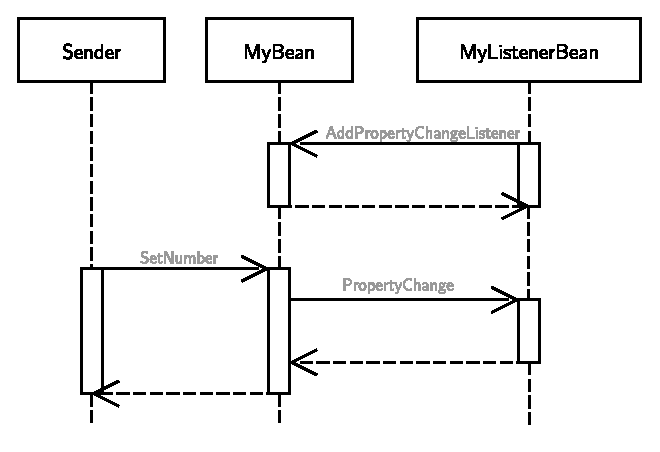
\includegraphics[scale=0.833]{src/javabeans}
%\end{center}

\section{Programmieridiome}
Ist eine abstrakte Schablone für ein konkretes Problem das sich für unterschiedliche Programmiersprachen unterschiedlich ausgestaltet.
\subsection{Objektgleichheit in Java}

\begin{enumerate}[leftmargin=*]\itemsep-2mm
    \item Prüfe, ob Argument eine Referenz auf aktuelles Objekt.
    \item Prüfe, ob Argument passenden Typ hat, mittels \texttt{instanceof} Operator ("`passend"' ist aktuelle Klasse, nicht die Basisklasse).
    \item Wende Typecast auf Argument an, um Referenz auf passenden Typ zu erhalten.
    \item Für alle (wesentlichen) Instanzvariablen des aktuellen Typs und möglicherweise von abstrakten Obertypen, prüfe Gleichheit (Referenz oder Identität).
    \item Prüfe, ob Implementierung in Schritt 4. eine Äquivalenzrelation (= 1. Reflexiv, 2. Symmetrisch, 3. Transitiv) definiert.
\end{enumerate}

\begin{minipage}{0.65\columnwidth}
\begin{lstlisting}[style=siemens, language=Java]
public final class TelefonNummer {
 private final short vorwahl;
 private final short rufnummer;
 //...
 public final boolean equals(Object o) {
  if(o==this)
    return true;
  if(!(o instanceof Telefonnummer)){
    return false;
    TelefonNummer t = (TelefonNummer)o;
    return t.vorwahl == this.vorwahl && 
    t.rufnummer == this.rufnummer; } } }
\end{lstlisting}
\end{minipage}\hfill%
\begin{minipage}[c][4cm]{0.3\columnwidth}
\rotatebox{90}{1. a.eq(a) == true}
\rotatebox{90}{2. a.eq(b) == b.eq(a)}
\rotatebox{90}{3. a.eq(b) und b.eq(c) == true}
\rotatebox{90}{dann: a.eq(c) == true}
\rotatebox{90}{Außerdem: a.eq(null) == false}
\rotatebox{90}{Methode \textbf{ohne} Seiteneffekte}
\end{minipage}

\subsection[Mixin]{Mixin \hfill \small \textcolor{siemensred}{mit Mehrfachvererbung} und \textcolor{siemensblue}{ohne Mehrfachvererbung}}

\begin{center}
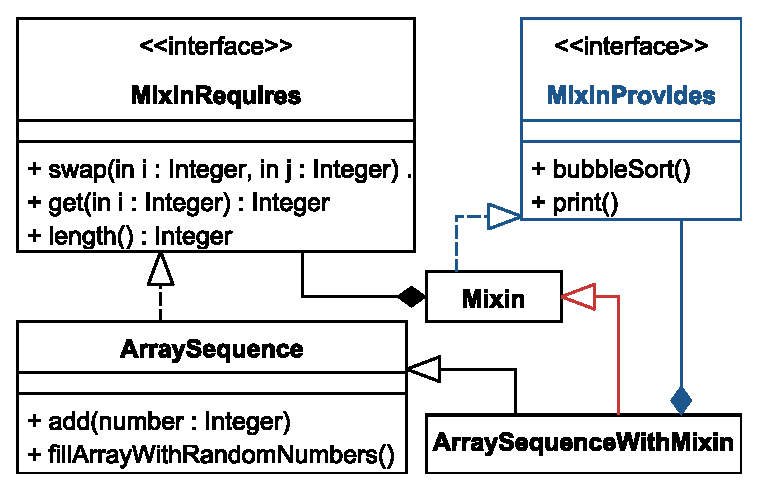
\includegraphics[width=0.85\columnwidth]{src/mixin}
\end{center}

\begin{description}[leftmargin=*]\itemsep-2mm
\item[Nutzen] Erweiterung der Klassenfunktionalität ohne Eingriff in die Vererbungshierarchie.
\item[\textcolor{siemensred}{Probleme}] Deadly Diamond of Death: Namenskonflikte (Welche Implementierung von gleichnamigen Methoden wird verwendet?), Werden Instanzvariablen 2 mal vererbt?
\item[Lösungsansatz] Verbiete diesen Fall, Selektive Replikation (Klasse gibt an, welche Instanzvariablen zu replizieren sind)
\end{description}

\begin{multicols}{2}

\section{Design Patterns}
\begin{description}[leftmargin=*]\itemsep-2mm
\item[Setzen] eine objektorientierte Softwareentwicklung vorraus
\item[Regeln] zur Lösung von häufigen Problemen bei der Softwareerstellung (abstrahieren, strukturieren, Lösung erarbeiten, Lösung abbilden).
\item[Katalysatoren] um Wiederverwendung, Formbarkeit und Modularität zu erreichen.
\item[Nutzen] Identifikation von wiederkehrenden Problemen und Dokumentation einer wiederverwendbaren Lösung (Diskussion Vor- Nachteile)
\end{description}
\end{multicols}
\subsection{Observer}
\paragraph*{Problem} Der Zustand mehrerer Objekte, die miteinander in Beziehung stehen, soll konsistent gehalten werden.
\begin{center}
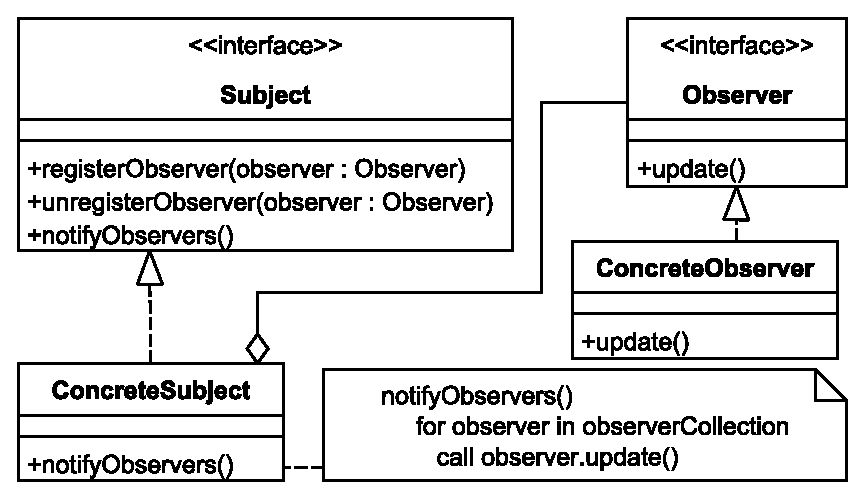
\includegraphics[width=0.85\columnwidth]{src/observer}
\end{center}


\begin{multicols}{2}
\textbf{Pro:}
\begin{itemize}[leftmargin=*]\itemsep-2mm
	\item Abstrakte Kopplung zwischen Subjekt und Beobachter
	\item Broadcast-Kommunikation an alle relevanten Objekte
\end{itemize}
\textbf{Contra:}
\begin{itemize}[leftmargin=*]\itemsep-2mm
	\item Nicht bekannt was verändert wird
	\item Kann viele Updates zur Folge haben
	\item unerwartete Änderungen
 \end{itemize}
		
		
\end{multicols}

Das Listener Pattern ist eine spezielle Umsetzung des Observer Patterns. Anstatt Aufruf einer \texttt{update()} Methode (Observer) werden aber Ereignisse generiert (Listener).

\subsection{Model View Controller (Architekturmuster)}
%\begin{center}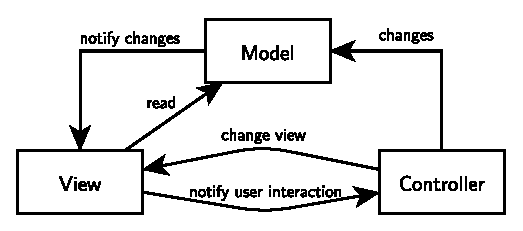
\includegraphics{src/mvc}\end{center}

\begin{description}[leftmargin=*]\itemsep-2mm
\item[Kontext] Interaktive Anwendung, die variable Daten in verschiedenen Sichten darstellt.
\item[Problem] Anforderungen an die Bedienoberfläche einer Anwendung können sich häufig ändern. Implementierung der Bedienoberfläche soll unabhängig vom funktionalen Kern der Anwendung veränderbar sein. Anwendungsdaten sind darstellbar durch verschiedene Sichten. Sichten sollen bei Datenänderung unmittelbar angepasst werden.
\item[Lösung] Die Implementierung einer interaktiven Anwendung soll in drei Bereiche aufgeteilt werden (Modularisierung).
\item[Model] (Data and Processing): Implementiert Kernfunktionalität und Datenmodell der Anwendung und ist unabhängig von Ausgabeformat und Eingabeverhalten. Registriert abhängige View und Controller Objekte und benachrichtigt diese bei Datenveränderung.
\item[View] (Output): Darstellung von Anwendungsdaten an der Benutzerschnittstelle. Fragt darzustellende Daten vom Modell ab. Verwaltet Controller Objekt(e). Kann Callback Methode implementieren, die bei Veränderung des Modells aufgerufen wird (Observer Pattern).
\item[Controller] Controller (Input): Wertet Benutzereingaben aus. Ruft Dienste im View Objekt oder Model Objekt auf in Abhängigkeit von der Benutzereingaben. Kann Callback Methode implementieren, die bei Veränderung des Model Objekts aufgerufen wird (Observer Pattern).
\item[Seperation of Concerns] Trennt die Verantwortlichkeiten für die Darstellung (View), die Verwaltung der Daten (Model) und die Kontrolle der Benutzereingaben bzw. der Änderung von Daten (Controller).
\item[Konsequenzen (+)] Mehrere Views je Datenobjekt (Model). Views werden automatisch konsistent gehalten (Observer Pattern). Keine Kopplung des Model mit View und Controller. View und Controller sind austauschbar (zu Laufzeit: pluggable). View und Controller (weil gelöst von Model) unabhängig wiederverwendbar. MVC Architektur kann mit abstrakten Basisklassen unterstützt werden.
\item[Konsequenzen (-)] Enge Kopplung zwischen View und Controller. Unabhängige Wiederverwendung von View und Controller ist nur selten möglich. Oft Trennung nicht sinnvoll und sorgt für unnötige Komplexität. Dennoch: Kopplung zwischen (View, Controller) und Model: View und Controller rufen Dienste von Model Objekten direkt auf. Es gibt ein Design Pattern das Abhilfe schafft (Command Pattern).
\end{description}

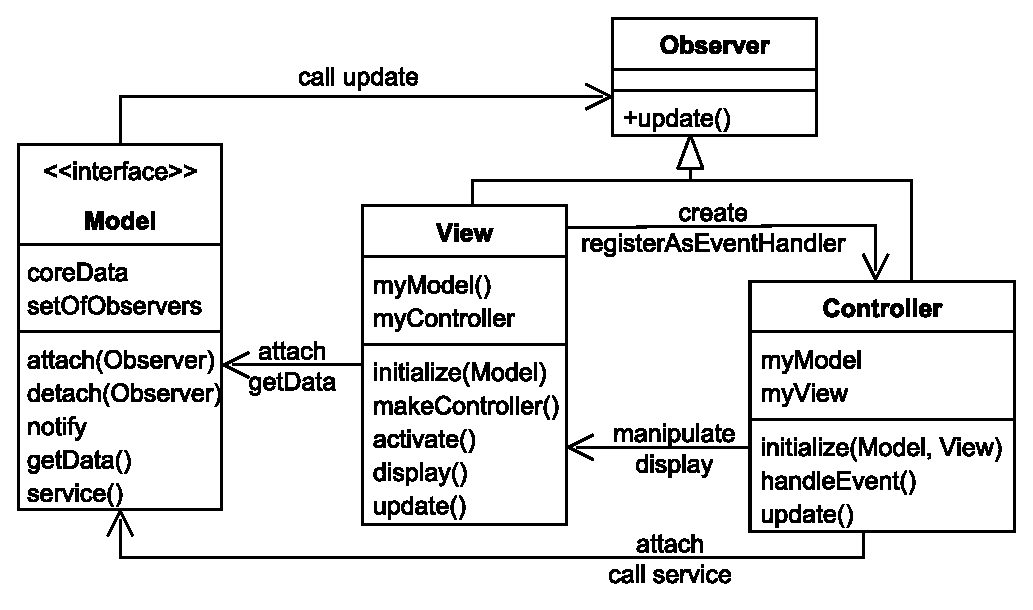
\includegraphics[width=\columnwidth]{new/mvcumlnew}

\subsection{Strategy}

\begin{minipage}{0.68\columnwidth}
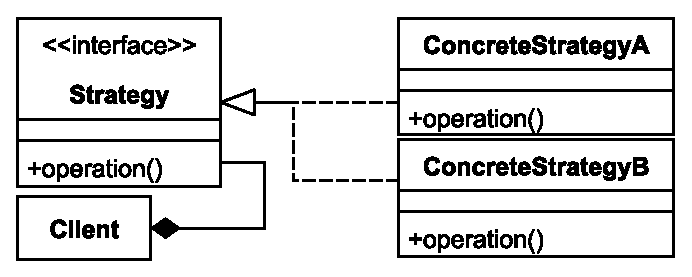
\includegraphics[width=\linewidth]{src/strategy}
\end{minipage}\hfill%
\begin{minipage}{0.3\columnwidth}
Das Strategy-Muster (Policy) definiert eine Familie von Algorithmen, kapselt sie einzeln und macht sie austauschbar. 
\end{minipage}
Es ermöglicht so, den Algorithmus unabhängig vom Client, der ihn einsetzt, variieren zu lassen


%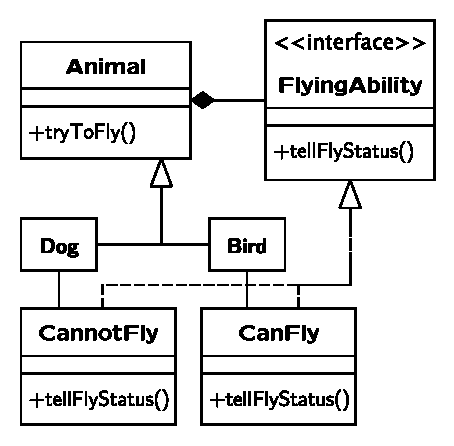
\includegraphics[scale=0.833]{src/strategy_bsp}

\begin{multicols}{2}
\textbf{Pro:}
\begin{itemize}[leftmargin=*]\itemsep-2mm
	 \item Familien von Algorithmen
	 \item Alternative zu Subklassen 
	 \item Eliminiert Abfragen und Verzweigungen
\end{itemize}
\textbf{Contra:}
\begin{itemize}[leftmargin=*]\itemsep-2mm
	 \item größere Anzahl von Objekten
	 \item Strategien müssen bekannt sein
	 \item Schnittstellen evtl. zu groß für simple Strategien
 \end{itemize}

\end{multicols}

\subsection{Iterator}
\begin{description}[leftmargin=*]\itemsep-2mm
\item[Problem] Elemente einer Container Datenstruktur aufzählen, ohne deren interne Datenstruktur zu kennen. Mehrere unabhängige Aufzählungen und verschiedene Reihenfolge soll möglich sein.
\item[Definition] Iterator-Muster bietet eine Möglichkeit, auf die Elemente in einem Aggregat-Objekt sequentiell zuzugreifen, ohne die zu Grunde liegende Implementierung zu offenbaren.
\item[Konsequenzen]  Schnittstelle der Container-Klasse wird einfacher, Zustand der Iteration ist unabhängig vom Container, Iteratoren mit verschiedenen Durchlaufstrategien sind denkbar. Verstößt gegen Law of Demeter!
\item[Realisierung] Wie verhält sich der Iterator bei Veränderung der unterliegende Datenstruktur?
\textbf{Wird invalidiert:} Exception bei aufruf von \texttt{hasNext()}, \texttt{next()}. "`Sieht"' Veränderungen \textbf{nicht} (Snapshot Iterator) bzw. "`Sieht"' Veränderung (mit Observer Pattern)
\end{description}

\begin{center}
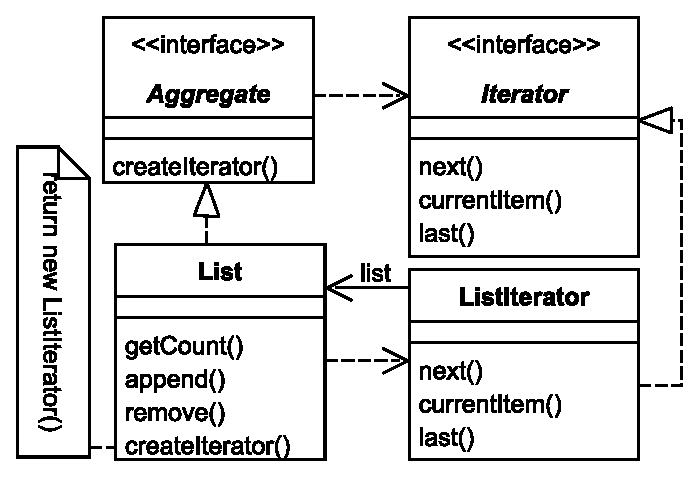
\includegraphics[width=0.85\columnwidth]{new/iteratoruml}
\end{center}

\subsection{Composite}

\begin{description}[leftmargin=*]\itemsep-2mm
\item[Motivation und Problem] Objekte (Whole-Part-Beziehung) sollen in einer hierarchischen Objektstruktur verwaltet werden. Clients sollen zusammengesetzte Objekte und einzelne Objekte gleich verwenden können.
\item[Lösung] Gemeinsame Schnittstelle (Component) für Kompositum und Blatt mit der Funktionalität: 1. Operationen, die zur Verwaltung der Objekthierarchie dienen. 2. Operationen, die Funktionalität eines einzelnen Bausteins in der Hierarchie betreffen.
\item[Konsequenzen] Client erkennt keine Unterschiede zwischen Kompositum und Blatt. Erweiterung um neuen Komponententypen: Neue Klasse implementiert Schnittstelle Component.
\end{description}


\begin{minipage}{0.38\columnwidth}
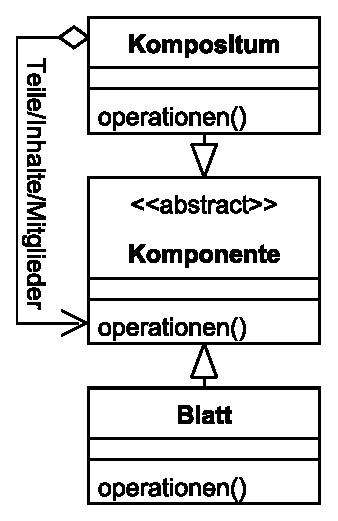
\includegraphics[width=\textwidth]{new/composite}
\end{minipage}\hspace{1mm}%
\begin{minipage}{0.6\columnwidth}
\begin{description}[leftmargin=*]

\item[Realisierung] Maximierung der Component-Schnittstelle für alle möglichen Elemente der Hierarchie evtl. problematisch, weil: Operationen nicht für alle Elemente sinnvoll sind. Es zwei Möglichkeiten zur "`Positionierung"' der Operationen zur verwaltung gibt (Definition und Deklaration in Klasse oder Deklaration in Schnittstelle, Implementierung in Kompositum, "`Dummy"' in Blatt Klassen)
\item[Negativ] Single-Responsibility-Prinzip \textbf{nicht} erfüllt! Wird der Rückwirkungsfreiheit (Aufrufe der gleichen Operationen auf Kompositum oder Blattknoten bleiben rückwirkungsfrei - ohne Nebeneffekte) geopfert. 
\end{description}

\end{minipage}

\subsection{Factory Method}
\begin{description}[leftmargin=*]\itemsep-2mm
\item[Problem] Ein Objekt soll erzeugt werden. Im Kontext ist nur die Schnittstelle, nicht aber die konkrete Klasse der zu erzeugenden Instanz bekannt. Nur abgeleitete Klassen kennen die konkrete Klasse.
\item[Konsequenzen] Factory Method bietet Hook für Subklasse, um Verhalten einer Methode in der Basisklasse zu konfigurieren. Product und Creator bilden häufig "`parallele"' Klassenhierarchien.
\item[Kritik an new] Code ist evtl. nicht gegen Veränderungen geschlossen.
\item[Verstößt] gegen Law of Demeter, was aber i.O. ist bei Objekterzeugung
\end{description}

\begin{center}
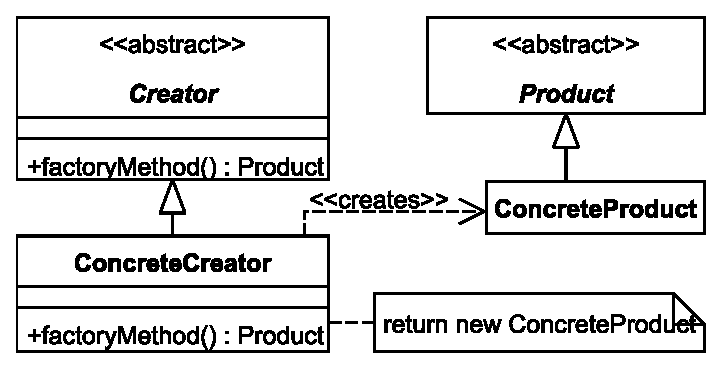
\includegraphics[width=0.85\columnwidth]{src/factory}
\end{center}

\subsection{Abstract Factory}
\begin{description}[leftmargin=*]\itemsep-2mm
\item[Problem] Objekterzeugung und Verwendung von diesen Objekten soll weiter entkoppelt werden. Factory Method legt Klasse der Objekte fest. Manchmal will man Objekte aus unterschiedlichen Klassen erzeugen.
\item[Lösung] Objekterzeugung wird an eigens dafür vorgesehenes Objekt delegiert. Factory Instanzen implementieren mehrere Factory Methoden die Objekte unterschiedlicher Klassen (aus der gleichen Familie) erzeugen.
\item[Realisierung] Schnittstelle der AbstractFactory sieht eine Factory Methode je Produkt vor. Pro Produktfamilie ist eine ConcreteFactory Klasse zu definieren
\item[Konsequenzen] System arbeitet unabhängig von Objekterzeugung. Austausch von Produktfamilien ist einfach. Schwierig, neue Produkte einzuführen, da alle Factoryklassen um eine Methode ergänzt werden müssen
\end{description}

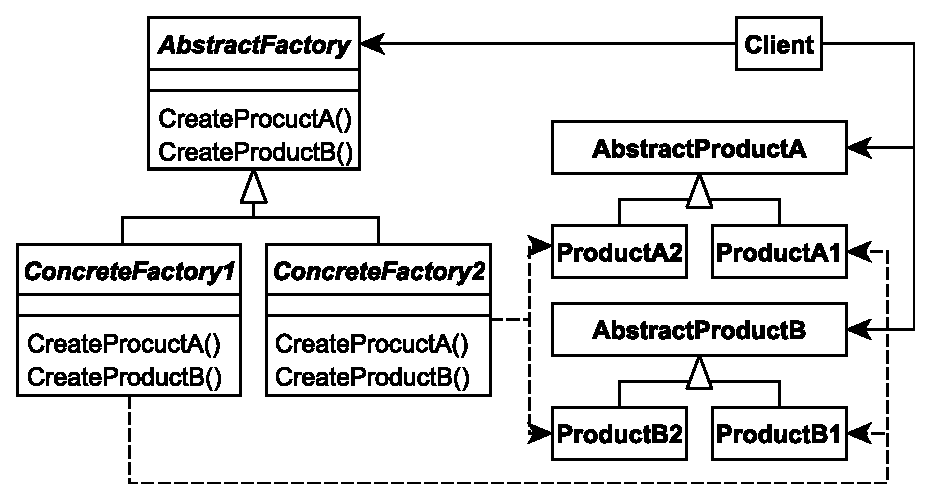
\includegraphics[width=\columnwidth]{new/abstractfactory}

\subsection{Adapter}
\begin{description}[leftmargin=*]\itemsep-2mm
\item[Motivation / Problem] Client erwartet eine bestimmte Schnittstelle zum Aufruf eines Services. Service Objekt bietet erwartete Funktionalität, aber Schnittstelle ist nicht kompatibel mit Client.
\item[Lösung] Entkopple Aufruf eines Services von der Realisierung des Services. Das Zwischenobjekt wird Adapter (Stellvertreter) genannt.
\item[Konsequenzen] Adapter kann neue Schnittstelle bereitstellen. Adapter soll mit Instanzen verschiedener Klassen (Adaptee und Subklassen) arbeiten. 
\item[Two-Way-Adapter] Clients erwarten unterschiedliche Schnittstellen: (voraussetzung: Mehrfachvererbung). TwoWayAdapter erbt von Target + Adaptee, kann so verschiedene Clients versorgen. 
\end{description}

\begin{center}
	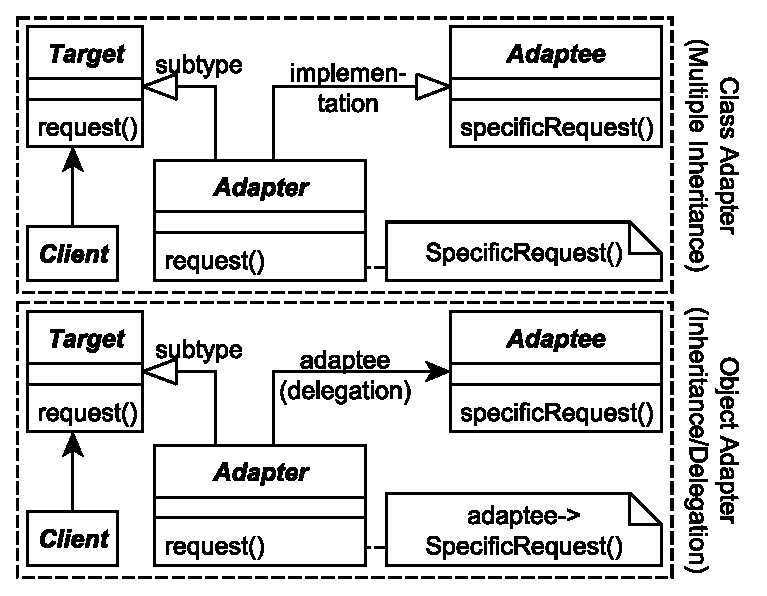
\includegraphics[width=0.85\columnwidth]{./new/adapter}
\end{center}

\subsection{Proxy}
\begin{description}[leftmargin=*]\itemsep-2mm
\item[Motivation / Problem] Erzeugung \& Initialisierung eines Service Objekts sei "`teuer"'. Objekt soll nur bei Bedarf erzeugt und initialisiert werden.
\item[Lösung] Entkopple Aufruf eines Services von der Realisierung des Services durch ein Zwischenobjekt. 
\item[Konsequenzen] Zusätzliche Indirektion zwischen Aufrufer und Objekt

\end{description}

\begin{center}
	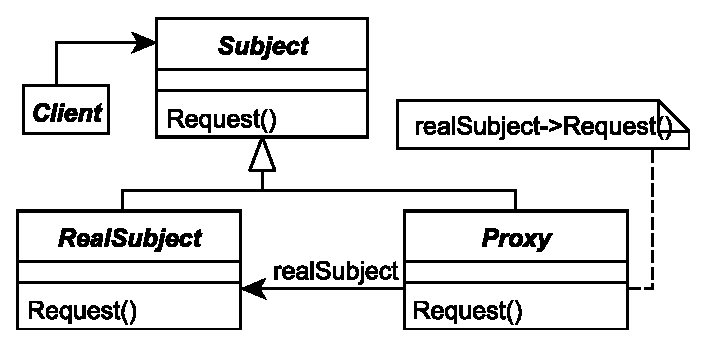
\includegraphics[width=0.80\columnwidth]{./new/proxy}
\end{center}

\subsection{Vergleich: Proxy / Adapter / Decorator}
\begin{description}[leftmargin=*]\itemsep-3mm
\item[Proxy] Implement gleiche Schnittstelle wie Service Objekt.
\item[Adapter] hat Schnittstelle, welche verschieden vom Service Objekt ist.
\item[Decorator] hat Schnittstelle, welche die des Service Objekts erweitert.
\end{description}



\begin{minipage}[h]{0.63\columnwidth}
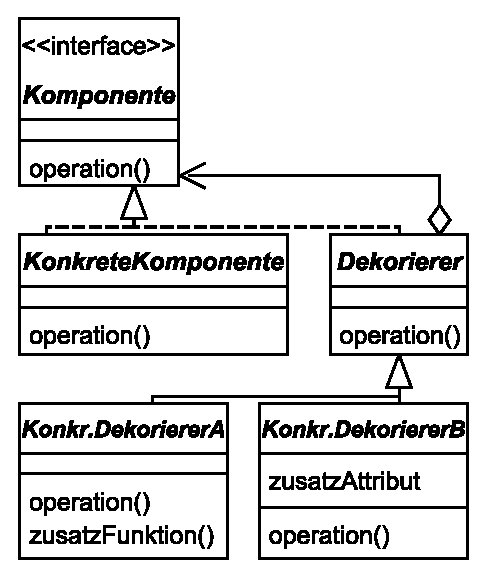
\includegraphics[width=\textwidth]{new/decorator}
\end{minipage}%
\hspace{-4.1cm}%
\begin{minipage}[h]{0.76\columnwidth}
\vspace{-5.5cm}%
\subsection{Decorator}
\begin{description}[leftmargin=*]
\item[Motivation / Problem] Funktionalität eines Objekts soll erweitert werden, ohne jedoch die Klasse des Objekts zu verändern. Nur bestimmte Instanzen der Klasse sollen die erweiterte Funktionalität implementieren.
\end{description}
\end{minipage}

\hspace{6.4cm}
\begin{minipage}[h]{0.37\columnwidth}
\vspace{-6.4cm}%
\begin{description}[leftmargin=*]
\item[Lösung] Kapsle Service Objekt in einem Decorator Objekt. Decorator implementiert gleiche Schnittstelle wie das ursprüngliche Objekt; erweiterte Schnittstelle optional. Implementierung des Decorators erweitert die Funktionalität hinter der ursprünglichen Schnittstelle und leitet letztlich Aufrufe an das gekapselte Objekt weiter.
\end{description}
\end{minipage}

\vspace{-0.55cm}
\begin{description}[leftmargin=*]\itemsep-2mm
\item[Konsequenzen] Decorator erweitert Funktionalität bzw. Verantwortlichkeit eines Objekts. Er vermeidet, dass "`zu viel"' Funktionalität in Basisklassen implementiert wird. Decorator kann zu vielen kleinen Klassen und Objekten führen: Schwer verständlicher Code, schweres debugging. Evtl. gehen Objekt-Identitäts-Tests falsch aus.
\item[Decorator vs Vererbung]  Flexibler als Vererbung, weil: Vererbung ist statisch, Vielfältige Kombinationen von Decorator und Service Objekten sind möglich. Decorator Objekt “kennt” Service Objekt nur durch Schnittstelle (Black-Box Reuse).
\item[Ähnlichkeit] Ist ein degeneriertes Composite-Pattern, d.h., es hat nur eine Komponente, das Service Objekt.
\item[Versus Strategy] Benutzt dieses min. ein mal: Client (=Dekorierer), Strategy-Interface (=Komponente) und StrategyA (=KonkreteKomponente). "`Strategy pattern changes the guts"', "`Decorator pattern changes the skin"'.
\end{description}


\subsection{Command}
\begin{description}[leftmargin=*]\itemsep-2mm
\item[Motivation / Problem] Eine Operation und deren Ausführungskontext sollen "`gespeichert"' werden, um: den Aufruf zu verzögern, die Wahl der Operation vom Aufruf der Operation zu entkoppeln, die Ausführung der Operation an anderer Stelle (anderer Thread) zu ermöglichen, mehrere Operationen zu gruppieren.
\item[Lösung] Kapsle Operation in einem eigenständigen Objekt
\item[Verhalten] Client erzeugt und initialisiert Command Objekt, Client registriert Command Objekt bei möglichen Aufrufern (Invoker), Aufruf einer Operation am Zielobjekt (Receiver) durch das Command Object via Callback (Invoker kennt Receiver nicht).
\item[Konsequenzen] Operationen sind in Command Instanzen gekapselt und können wie "`normale"' Objekte verwaltet werden. Command Objekte können Zustand haben (z.B. Argumente)
\end{description}

\begin{center}
	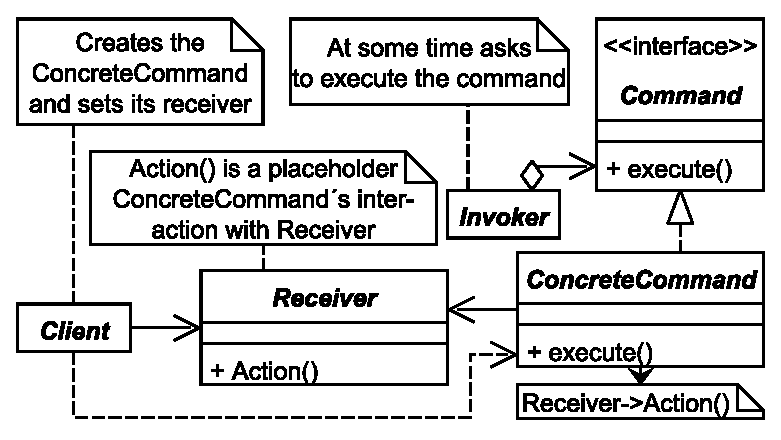
\includegraphics[width=0.85\columnwidth]{./new/command}
\end{center}

\begin{multicols}{2}
\subsection{Facade}
\begin{description}[leftmargin=*]\itemsep-2mm
\item[Motivation / Problem] Subsystem hat eine Vielzahl von Schnittstellen, Client verwendet mehrere davon. Dadurch erhöhte Komplexität im Client und viele Abhängigkeiten. 
\item[Lösung] Fasse Schnittstellen, die ein spezieller Client verwendet, in einem Facade Objekt zusammen.
\item[Konsequenzen] Vereinfachung der Schnittstelle und Entkopplung von den Schnittstellen der Subysteme (können dadurch unabhängig vom Client variieren). Client kann, muss aber nicht Schnittstellen des Subsystems verwenden. 
\end{description}
\end{multicols}

\begin{minipage}{0.29\linewidth}
\subsection{Singleton}
\begin{description}[leftmargin=*]
\item[Problem] Es soll nur eine Instanz einer bestimmten Klasse geben. Es soll nur einen globalen Mechanismus geben, über den die Instanz der Klasse abgerufen werden kann
\item[Lösung] Klasse selbst ist verantwortlich Ihre eigene Instanz zu verwalten $\rightarrow$ statische Methode getInstance()
\end{description}

\end{minipage}\hspace{1mm}%
\begin{minipage}{0.70\linewidth}
\begin{lstlisting}[style=siemens, language=Java]
public class S1 { //statische initialisierung
 private static S1 uniqueInstance = new S1();
 private S1() { //... }
 public static S1 getInstance() {
  return uniqueInstance; } }
public class S2 { //dynamische initialisierung
 private static S2 uniqueInstance= null;
 private S2() { //... }
 public static /*#here#*/ S2 getInstance() {
/* add synchronized #here# for thread safety */
 if(uniqueInstance == null)
  uniqueInstance = new S2();
 return uniqueInstance; } }
public class S3 { //implicit thread safety
 private static class SHolder {
  static final S3 uniqueInstance = new S3(); }
 public static S3 getInstance() {
  return SHolder.uniqueInstance; } }
\end{lstlisting}
\end{minipage}




\begin{multicols}{2}
\section{Architekturmuster}
\begin{description}[leftmargin=*]\itemsep-2mm
    \item[Beschreibt] Struktur + Organisation einer Anwendung (auf höchster Abstraktionsebene). Beschreibt die Menge vordefinierter Subsysteme, spezifiziert deren Zuständigkeit und enthält Regeln zur Organisation der Beziehungen zwischen ihnen. Sie sind prinzipiell sprachneutral und plattformunabhängig
\item[Voraussetzung] modulare Softwareentwicklung 
\end{description}

\subsection{Pipes and Filters}
(Ggf. parallele) Verarbeitung von Datenströmen in Komponenten
\begin{description}[leftmargin=*]\itemsep-2mm
\item[Filters (coroutines)] Unabhängige Komponenten zur Datenverarbeitung mit Input und Output. Operationen werden durch den Datenfluss gesteuert. 
\item[Pipes (streams)] Kanal, über den Daten vom Ausgabeport eines Filters zum Eingabeport des nächsten Filters geleitet werden.
\item[Implementierung] Filter haben bei strenger Auslegung des Musters keine Möglichkeit auf gemeinsame Daten zuzugreifen
\item[Varianten] Pipeline (strikt lineare Abfolge von Filtern) oder mit Fork/Join und Rückkopplung
\end{description}
%\includegraphics[width=\linewidth]{src/pipesfilters}

\end{multicols}


\begin{multicols}{2}

\section{Architektursichten}

\begin{description}[leftmargin=*]\itemsep-2mm
\item[Beschreibung] einer Softwarearchitektur kann gegliedert werden in
verschiedene Sichten (Architektursichten)
\item[Beschränkt] die Darstellung auf bestimmte Aspekte eines Softwaresystems. Vergleichbar mit Teilplänen eines Gebäudes (Mauerwerk, Elektro, Wasser, Heizung, Möblierung ...)
\item[Zur umfassenden Beschreibung] sollten alle Sichten dokumentiert werden
\end{description}

\subsection{4+1 Modell nach Kruchten}
\begin{description}[leftmargin=*]\itemsep-2mm
\item[Konzeptionelle Sicht] (Logical View) Dokumentiert Basiskomponenten + Kommunikationsbeziehungen
\item[Modulsicht] (Development View) Strukturbeschreibung der Implementierung eines Systems in Modulen (Klassen) + Subsystemen (Paketen). Keine Konfiguration, weil Kombination von Modulen für ein best. Produkt nicht beschrieben wird
\item[Ausführungssicht] (Process View) Beschreibt Instanziierung von Modulen zur Laufzeit (in spez. Systemkonfig)
\item[Programmsicht] (Physical View) Beschreibt Struktur von Dateien und Verzeichnissen eines Systems und deren Abhängigkeiten im Build-Prozess
\item[Kritik] Aspekte sind sehr allgemein. Beschreibt konkrete Architekturen, nicht deren Ableitung oder Zusammenhang in einem Architekturstil.
\end{description}
\end{multicols}

\begin{center}
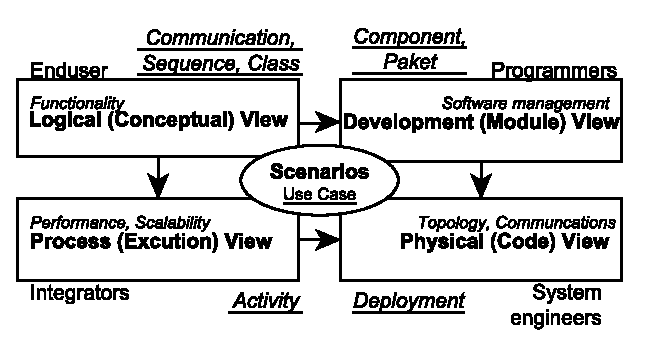
\includegraphics[width=0.95\columnwidth]{src/4+1}
\end{center}

\begin{multicols}{2}
\section{Clean Code}
\subsection{Namen}
\begin{description}[leftmargin=*]\itemsep-2mm
    \item[Keine Desinformationen] \texttt{Account\-List} nur, wenn es wirklich eine \texttt{List} von Acc(ounts) ist
    \item[Keine \textit{noise words}] wie \texttt{Info, Data, variable, table, string}
    \item[Auffindbare Namen] Einbuchstaben-Namen und numerische Konstanten sind praktisch nicht auffindbar
    \item[Namenslänge] proportinal zur Größe des Scopes
    \item[Vermeiden von Gehirnjogging] 
    \item[Klassennamen] Substantive oder Substantivierungen
    \item[Methodennamen] Verben oder Verbkonstruktionen, Accessors mit Präfix \texttt{get, set, is}
		\item[Zweckmäßigkeit] Namen von Variablen, Methoden oder Klassen sollen ihren Zweck verdeutlichen
		\end{description}

\end{multicols}
\begin{multicols}{2}

\subsection{Funktionen}
\begin{description}[leftmargin=*]\itemsep-2mm
    \item[Funktionen lesbar] von oben nach unten, wie ein Roman
    \item[Nur eine Aufgabe] und die wird möglichst gut gemacht
    \item[Möglichst wenige Parameter] (idealerweise)
    \item[Möglichst mit Exceptions] ohne Fehlerrückgabe (keine Fehlercodes)
    \item[Kein Flagparameter] da Funktion sonst oft mehr als eine Sache tut
		\item[Query] hat einen Rückgabewert und keine Seiteneffekte
		\item[Command] modifiziert das System und hat keinen Rückgabewert
		\item[Command-Query-Seperation], d.h. entweder oder
		\item[try/catch] Fehlerbehandlung ist eine Sache, Methode sollte daher vor \textbf{try} und nach \textbf{catch} keinen Code haben
\end{description}

\end{multicols}
\begin{multicols}{2}

\subsection{Allgemein}
\begin{description}[leftmargin=*]\itemsep-2mm
	\item[Principle of Least Astonishment] Methoden implementieren Verhalten, dass man erwartet
	\item[Toten Code] vermeiden (Code der nie ausgeführt wird, z.B. in if- oder catch-Block)
	\item[Code] auf einer Abstraktionsebene
	\item[Keine] Vererbung von Konstanten oder \textbf{public} Instanzvariablen (statt dessen private + Accessors)
	\item[Vertikale Entfernung minimieren] (Variablendefinition bei, Methoden nach erster Verwendung)
	\item[Überführen] von logischen (Modul A macht Annahme über Modul B) in technische Abhängigkeiten (Modul A erhält Member B)
	\item[fail fast] (Fehler so bald wie möglich erkennen)
	\item[Failure Atomicity] Aufrufe, der Fehler verursachen, belassen das Obj. in seinem Zustand
	\item[Checked Exceptions] für wiederherstellbare Konditionen. Möglichst vermeiden, liegen außerhalb der unmittelbaren Kontrolle des Programms
	\item[Unchecked Exceptions] für Programmierfehler, Unterklasse von Checked Exceptions (IllegalArgument, Nullpointer, ...)
	\item[Checked nach Unchecked] Methode in 2 Teile: eine generiert bool-Rückgabewert, wenn Exception generiert worden wäre
	\item[Enumerationen] statt Konstanten
	\item[Boilerplate Code] ist wiederkehrender Code der vermieden werden sollte
	\item[Nicht null] als Rückgabewert, sondern leere Arrays oder Collections
\end{description}

\end{multicols}
\begin{multicols}{2}

\subsection{Kommentare}
\begin{description}[leftmargin=*]\itemsep-2mm
	\item[Widmen sich] sich ausschließlich dem Code und der Architektur aus technischer Sicht
	\item[Kommentare für] Klarstellung-en, Warnungen, ToDos
	\item[Keine Redundanzen] an Informationen \texttt{i++ //increment i}
	\item[Auskommentierten Code] entfernen (Notfalls über Versionierungssystem wiederherstellen)	
	\item[Keine Informationen über] Issue-Tracking, Änderungshistorie und Metadaten (Autor, Änderungsdatum) 
\end{description}

\end{multicols}
\begin{multicols}{2}

\subsection{Javaspezifisches}
\begin{description}[leftmargin=*]\itemsep-2mm
\item[Wildcards] statt langer Importlisten
\item[Implementierung von] \texttt{toString()} und wenn \texttt{equals()}, dann auch \texttt{hashCode()}
\item[Enums] statt Konstanten verwenden
\item[Vermeiden sie Finalizers], (also Aufruf der Methode \textit{finalize}), da unvorhersagbar, häufig gefährlich und unnötig
\end{description}
\end{multicols}
\begin{multicols}{2}

\subsection{minimale Veränderbarkeit}
\begin{description}[leftmargin=*]\itemsep-2mm
	\item[Motivation] Vermeidung von Fehlerquellen, Sicherheitslücken schließen
	\item[Keine Methoden] die den Zustand eines Objekts verändern (Mutators/Setters), Getter ist i.O.
	\item[Subclassing verbieten] durch 1. \texttt{final} und 2. alle Konstruktoren private + \texttt{public static}-Fabrikmethode
	\item[Alle Instanzvariablen] als \texttt{final} und \texttt{private} deklarieren
	\item[Veränderbare Objekte] nicht zur Verfügung stellen
	\item[Defensive Kopien], d.h. keinen Zugriff auf Referenzen veränderbarer Objekte geben (bei getter oder Konstruktor)
\end{description}
\end{multicols}
\begin{lstlisting}[style=siemens, language=Java]
public final class Complex {
 private final double re; private final double im;
 private Complex(double re, double im) {  this.re = re;  this.im = im; }
 public static Complex valueOf(double re, double im) {
  return new Complex(re, im); } }
\end{lstlisting}

\section{UML}

\subsection{Klassische UML}
\vspace{-1.3cm}
\begin{center}

\begin{minipage}{0.7\linewidth}\vspace{1cm}
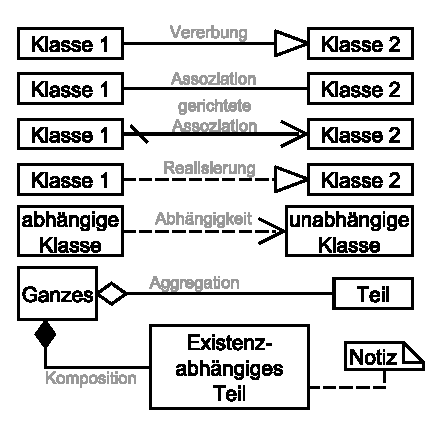
\includegraphics[width=\linewidth]{src/uml_klassen_delegation}
\end{minipage}\hfill%
\begin{minipage}{0.29\linewidth}
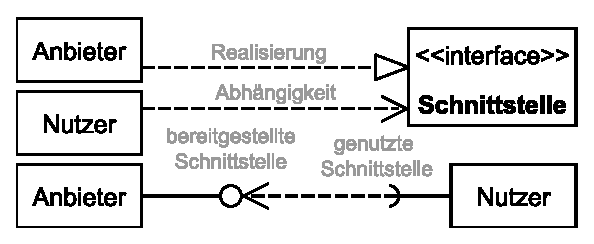
\includegraphics[height=\linewidth, angle=90]{src/uml_schnittstellen}
\end{minipage}

\end{center}



\begin{multicols}{2}

\subsection{Beschreibung innerhalb}
Sichtbar Name : Typ = Initialwert\\
Sichtbar Name (Params) : Rückgabe\\
Sichtbar: + public, \# protected, - private
Params: Name: Typ = Standardwert
\section{Komponentendiagramm}

\subsection{Anwendungsbereiche}
\begin{description}[leftmargin=*]\itemsep-2mm
\item[Eignet] sich für die Spezifikation von Softwarearchitekturen
\item[Entwurfsphase] Verteilung der Aufgaben großer Softwaresysteme auf kleinere Subsysteme. Häufig wird 3-Schichten-Architektur gewählt:
	\begin{description}[leftmargin=*]\itemsep-2mm
	\item[Datenspeicherung] wird einem Datenbankmanagementsystem überlassen
	\item[Geschäftslogik] wird durch eine Applikationsschicht erledigt
	\item[Präsentation + Benutzerinteraktion] werden in einer Präsentationschicht durchgeführt
	\end{description}
	\item[Nach der Definition] der einzelnen Komponenten und ihrer Aufgaben sowie deren Kommunikation kann die Entwicklung auf unterschiedliche Personen oder Entwicklerteams aufgeteilt und somit die Phase der Implementierung eingeleitet werden
	\item[Die Dokumentation] von Softwarekomponenten und Schnittstellen kann in der Test-
Phase als Grundlage von Integrationstests verwendet werden
\end{description}
\end{multicols}

\begin{multicols}{2}
\subsection{Verschiedene Elemente}
\begin{description}[leftmargin=*]\itemsep-2mm
\item[Eine Komponente] (engl. Component) repräsentiert einen ersetzbaren modularen Bestandteil eines Systems, das sein Inneres kapselt. Sie kann eine Ansammlung weniger Klassen bis hin zu großen Softwaresystemen repräsentieren
\item[Ein Bauteilkonnektor] (engl. Assembly Connector) stellt eine Verbindung zwischen zwei Bauteilen dar und spezifiziert, dass ein Bauteil Dienste eines anderen Bauteils in Anspruch nimmt
\item[Ein Delegationskonnektor] (engl. Delegation Connector) stellt eine Verbindung zwischen den externen Schnittstellen oder Ports und den inneren Bestandteilen einer Komponente dar
\item[Ein Artefakt] (engl. Artifact) repräsentiert eine physische Informationseinheit, die beim Softwareentwicklungsprozess verwendet oder hergestellt wird
\item[Manifest] verbindet ein Artefakt mit einer Komponente (gestrichelte Linie + Pfeil auf Komponente)
\end{description}
\subsection{Überführung aus Klassendiagramm}
\begin{description}[leftmargin=*]\itemsep-2mm
	\item[Komposition] axistenzabhängiger Teil wird Interna seines Ganzen
	\item[Realisierung] auf Interface wird Lolly
	\item[Abhängigkeit] auf Interface wird Halbmond
	\item[Beschriftung] Interfacename an beiden Seiten, Bauteilkonnektor dazwischen (gestrichelt, Pfeil auf Lolly)
	\item[Ports / Delegation] Benutzt eine interne Komponente ein Interface das von einer äußeren Komponente bereitgestellt wird benutzt man den Delegationskonnektor (durchgezogen, Pfeil in Richtung Lolly).
\end{description}
\end{multicols}

\begin{center}
	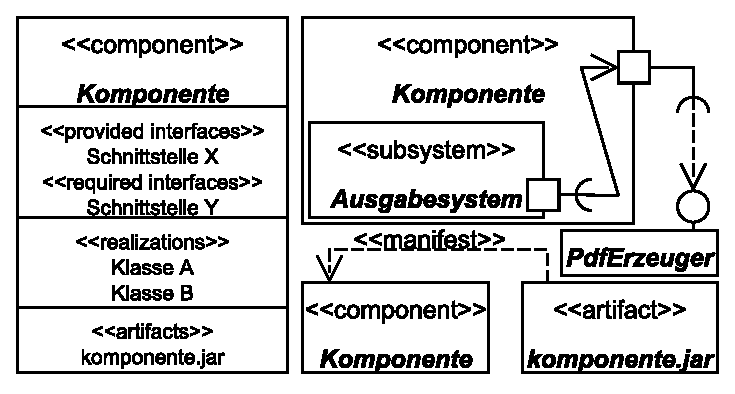
\includegraphics[width=0.95\linewidth]{new/komponentendiagramm}
\end{center}

\end{multicols}



\end{document}